\subsection{Trigger}
\label {sec:trigger}

The LHC beam crossing interval of 25 ns corresponds to a crossing
frequency of 40 MHz.  In addition, the nominal total size in memory required
to store all of the readout for a single CMS event is about 1.5 MB.
This corresponds to a data production rate of 40 TB per second, which is far 
too much to store and process.  To resolve this issue, CMS uses an online trigger
system to select only approximately one out of every $10^6$ events for storage
and processing.  This selection is divided between two components:
the Level 1 Trigger (L1), 
\nomenclature{L1}{Level 1 trigger} 
which reduces the event rate to a maximum of 100 kHz,
and the High Level Trigger (HLT)
\nomenclature{HLT}{High level trigger}
which further reduces the event rate to $\mathcal{O}(100\text{ Hz})$.
The final rate is meant to allow as inclusive a selection as possible while remaining 
within the limits of data recording technology.
For comparison purposes, the production rates in Hz of various processes (including scalar leptoquarks) 
assuming nominal beam energy and instantaneous luminosity
are shown in Figure \ref{fig:trigger-xsections}.

\begin{figure}
  \centering
  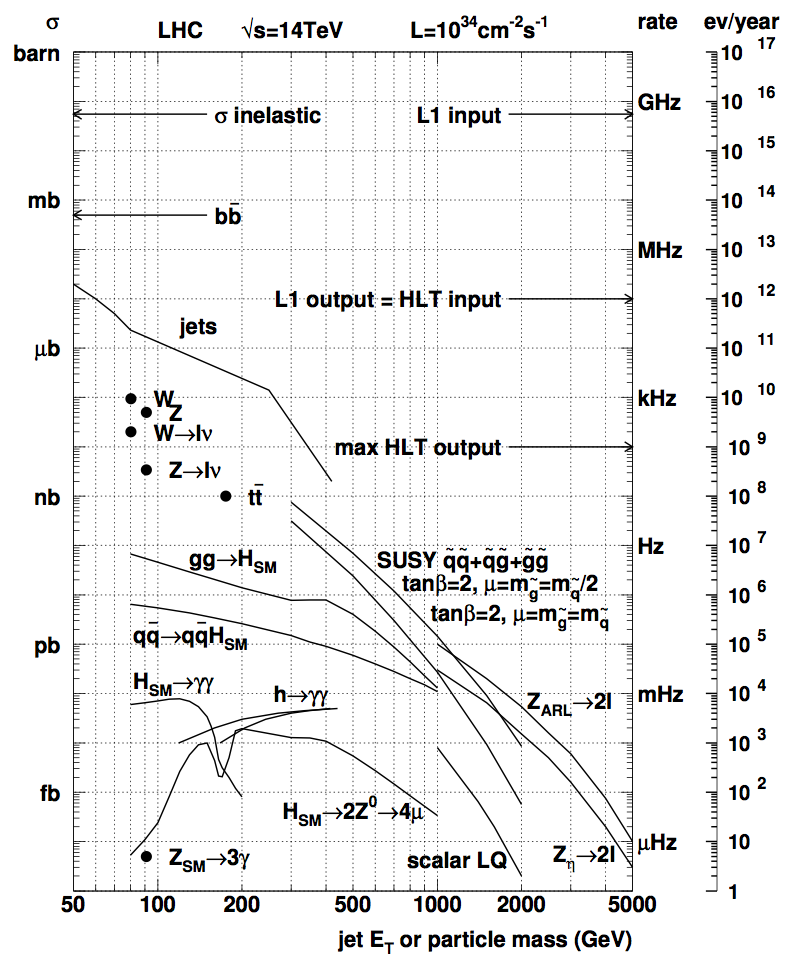
\includegraphics[width=0.95\textwidth]{tex/cms/fig/trigger-xsections.png}
  \caption{Production rates and cross sections associated with various 
    processes (including scalar leptoquarks) 
    in the LHC at design beam energy and luminosity. 
    For comparison purposes, the L1 and HLT input and output rates are shown.  
    It should be noted that the maximum HLT output rate quoted in this diagram (100 Hz) 
    is not a hard maximum.  Indeed, the HLT maximum output rate was around 300 Hz 
    during stable beams in 2011 running \cite{cms-jinst}.}
  \label{fig:trigger-xsections}
\end{figure}

The L1 is composed of custom-designed, largely programmable electronics 
housed partly on the detector itself and partly in a counting room 90m away from the detector.
The hardware is composed of field programmable gate arrays (FPGAs)
\nomenclature{FPGA}{Field programmable gate array}
where possible, but application-specific integrated circuits (ASICs)
\nomenclature{ASIC}{Application-specific integrated circuit}
and largely programmable look up tables (LUTs) 
\nomenclature{LUT}{Look up table}
are used where speed, density, or radiation hardness is required.
The L1 has access to coarsely segmented data from the calorimeters and the muon systems.
This data is processed in three components: local, regional, and global.
The local component is made up of Trigger Primitive Generators (TPGs)
\nomenclature{TPG}{Trigger primitive generator} which collect information
on energy deposits in the calorimeters and track segments or hit patterns in the muon chambers.
The regional component combines the local trigger primitives and uses pattern logic to 
rank and sort the resulting trigger objects (e.g. muon, electron, and jet candidates in limited regions of the detector).
In this context, ``rank'' is a function of the measured energy or momentum of a trigger object and 
the uncertainty associated with that measurement.
The global component consists of the Global Calorimeter Trigger (GCT)
\nomenclature{GCT}{Global calorimeter trigger}
and the Global Muon Trigger (GMT).
\nomenclature{GCT}{Global muon trigger} 
The GCT and GMT
collect the highest rank calorimeter and muon objects 
and transfer them to the Global Trigger (GT), 
\nomenclature{GT}{Global trigger}
where the decision to
accept the event and pass it on to the HLT is made.  
This decision is based on detector algorithms and on the readiness
of the data acquisition framework (DAQ), 
\nomenclature{DAQ}{Data acquisition framework}
as determined by the Trigger Control System (TCS).
\nomenclature{TCS}{Trigger control system}
The L1 Accept 
decision (L1A) \nomenclature{L1A}{Level 1 accept} is passed from the GT to the detector
subsystems via the Timing, Trigger, and Control system (TTC).
\nomenclature{TTC}{Timing, trigger, and control system}
The allowed latency for the L1 between a bunch crossing and the distribution of the trigger
decision to the detector electronics is 3.2 $\mu$s.  During this latency period,
the full resolution data from the detector is stored in pipeline memories in the front end electronics.
A logical schematic of the L1 architecture is shown in Figure \ref{fig:trigger}.

\begin{figure}
  \centering
  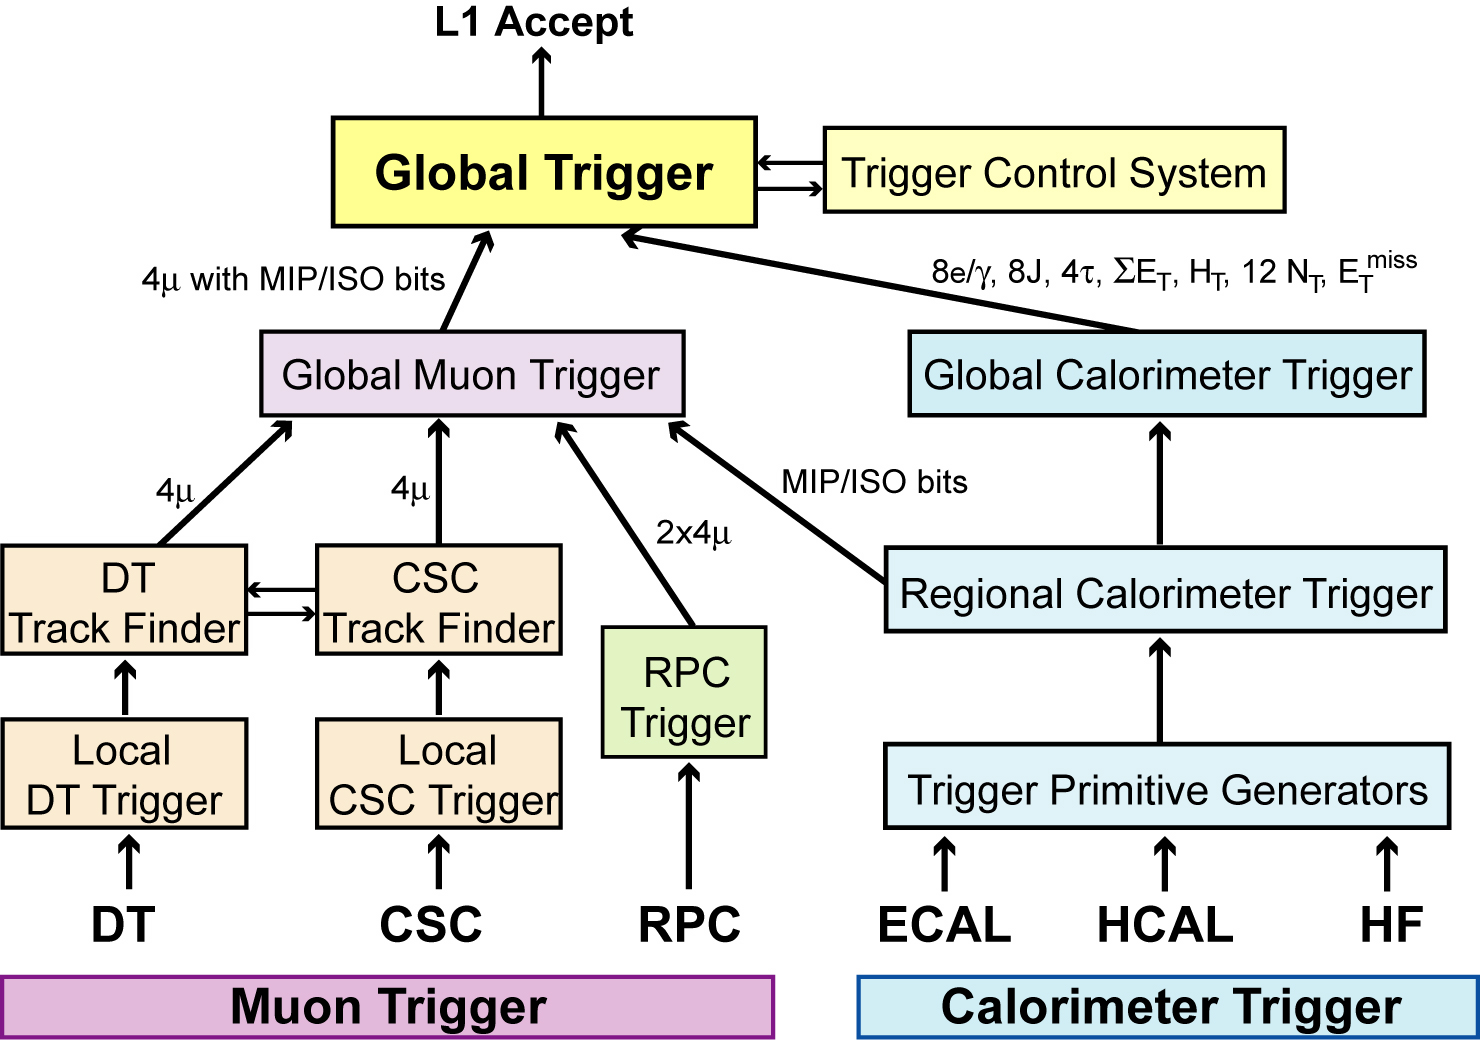
\includegraphics[width=0.6\textwidth]{tex/cms/fig/trigger-schematic.jpg}
  \caption{Logical schematic of the architecture of the Level 1 Trigger (L1) \cite{cms-jinst}}
  \label{fig:trigger}
\end{figure}

The HLT \cite{hlt} is software system implemented on a farm of commercially 
available CPUs.  
Unlike the L1, the HLT
has access to the full detector readout and can make complex calculations
comparable to those available in a fully offline analysis.
Furthermore, the CMS software framework (CMSSW) \nomenclature{CMSSW}{CMS software}
used by the HLT is essentially
the same framework used for offline analysis.
The HLT selects events using a list of triggers which are written as software algorithms.  
A common HLT algorithm is to select an event with a trigger object above a given
transverse momemntum or energy threshold.  These trigger objects 
may include single objects, for example: electrons, muons, taus, jets, or photons.  They
may also include composite objects, for example: \met, or dilepton invariant mass.
The HLT may also pass through some L1 decisions for the purpose of detector study or calibration.
The full list of triggers is refered to
as the HLT ``trigger menu''.  Events accepted by a trigger are sorted into 
primary datasets (PDs) \nomenclature{PD}{Primary dataset}
and written to storage. 
Some triggers are configured to accept every event that passes their selection requirements.
Other triggers only take one out of every $N$ events that pass. 
The former triggers are known as ``unprescaled'' triggers. The latter
triggers are known as ``prescaled'' triggers, and  $N$ is known as the ``trigger prescale''.
Triggers with similar selection topologies
are grouped together and their outputs are written to the same PD, in order 
to minimize the overlap between various PDs.  
Because the HLT is entirely software-driven, the trigger menu is extremely 
flexible and has the ability to change with evolving conditions at the LHC 
\cite{cms-tdr,cms-jinst}.
